% Asset ID: AS1DifferentiationTIKZ-001
% Source: Chapter 12 Differentiation PDF p.3 + CCEA AS1-DIFF-LO001
% Related lesson section: Core Theory 1
% Purpose: Show y=x^2 with tangent gradients and the gradient function dy/dx=2x.

\documentclass[tikz,border=8pt]{standalone}
\usepackage{amsmath}
\usepackage{pgfplots}
\pgfplotsset{compat=1.18}

\begin{document}
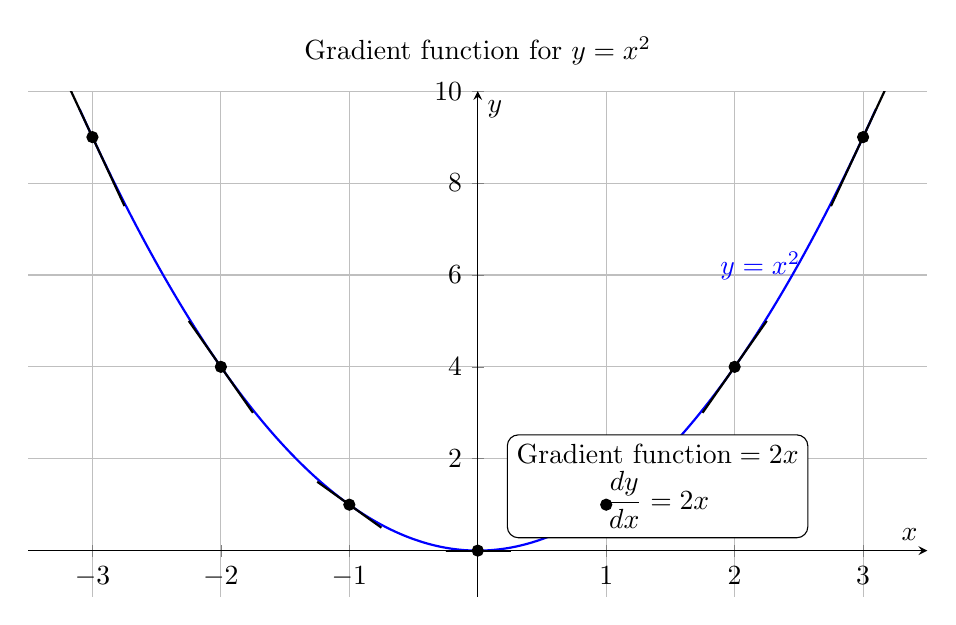
\begin{tikzpicture}
\begin{axis}[
    width=13cm,
    height=8cm,
    axis lines=middle,
    xmin=-3.5, xmax=3.5,
    ymin=-1, ymax=10,
    grid=both,
    xlabel={$x$},
    ylabel={$y$},
    title={Gradient function for $y=x^2$},
    samples=200,
    domain=-3.1:3.1
]
\addplot[thick, blue] {x^2};
\node[blue] at (axis cs:2.2,6.2) {$y=x^2$};

\foreach \a/\m in {-3/-6,-2/-4,-1/-2,0/0,1/2,2/4,3/6} {
    \addplot[black, thick, domain=\a-0.25:\a+0.25] {\m*(x-\a)+\a*\a};
    \addplot[only marks, mark=*, black] coordinates {(\a,\a*\a)};
}

\node[fill=white, draw, rounded corners, align=center] at (axis cs:1.4,1.4)
{$\text{Gradient function}=2x$\\[2pt]$\displaystyle \frac{dy}{dx}=2x$};

\end{axis}
\end{tikzpicture}
\end{document}
